\section{Durchführung}
\label{sec:Durchführung}
%@Rene: Wenn dir ein besserer Name als "Schaltplatte" einfällt, kannst du diesen gerne ersetzen 
Alle Messungen werden mit der in Abbildung \ref{fig:platte}
gezeigten Schaltplatte durchgeführt. 
\begin{figure}
    \centering
    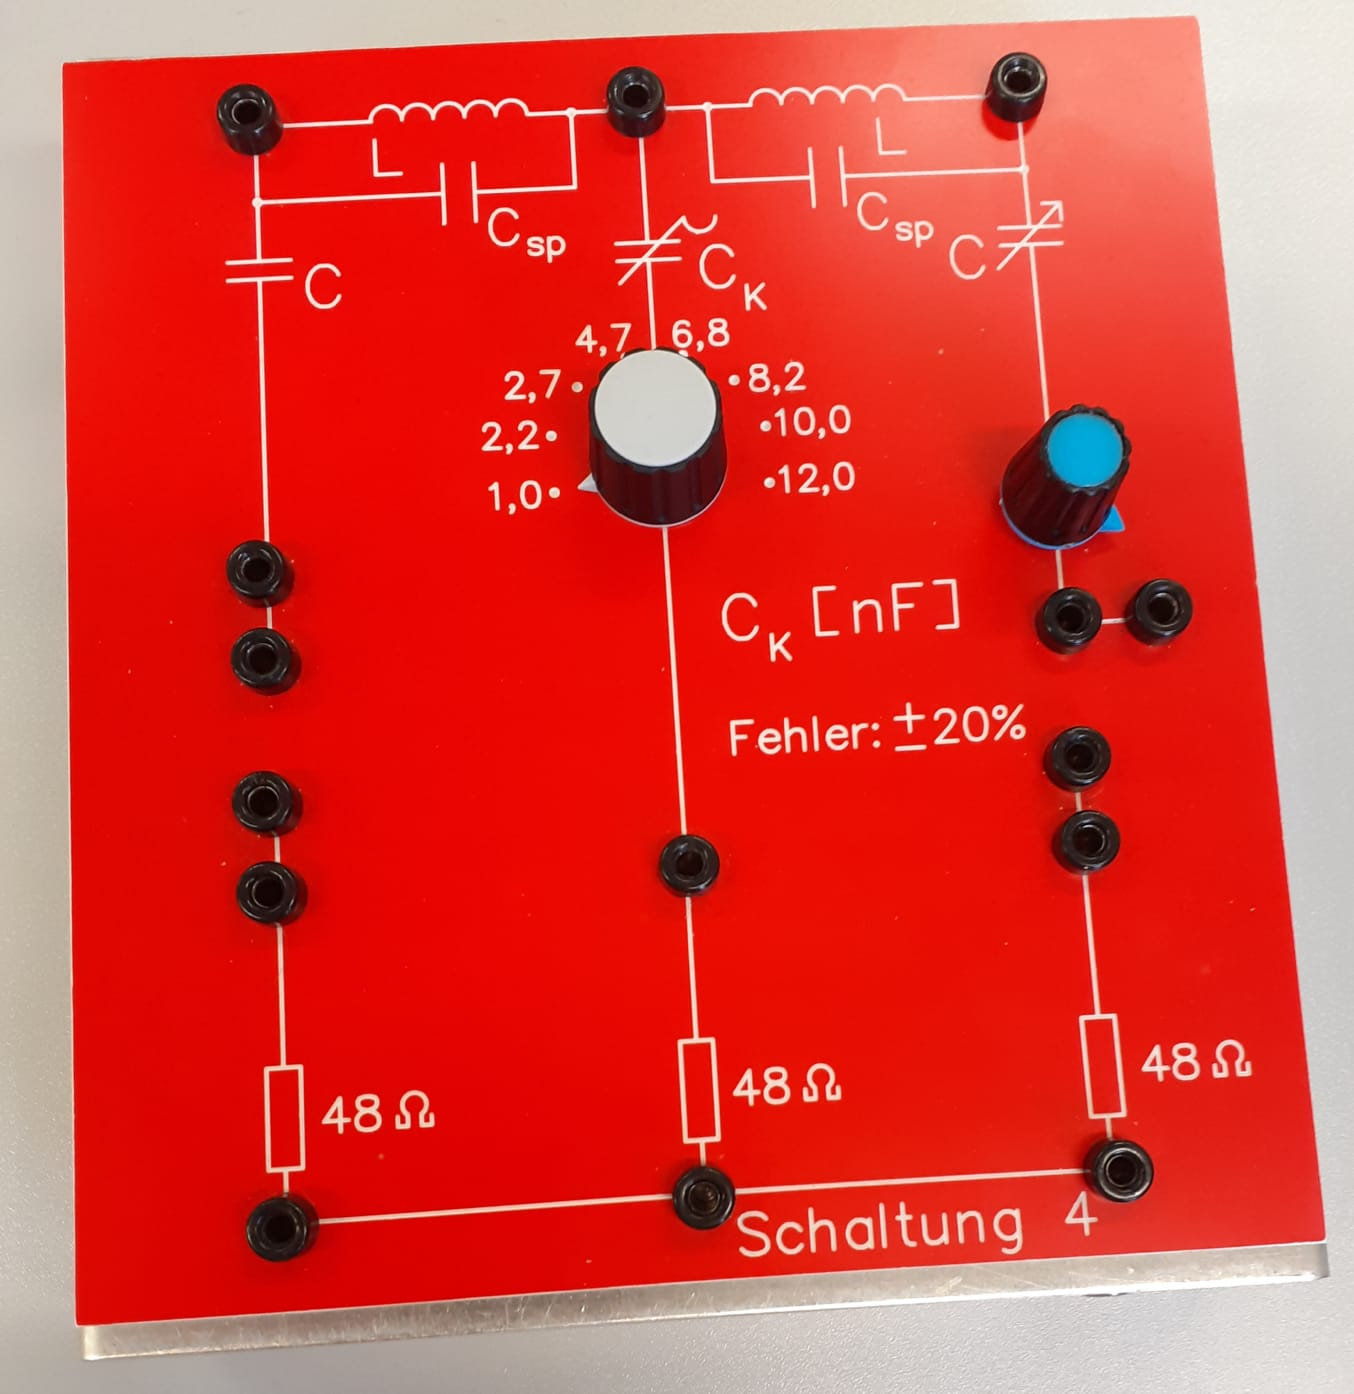
\includegraphics[width=0.5\textwidth]{plots/Platte.jpeg}
    \caption{Die verwendete Schaltplatte.}
    \label{fig:platte}
\end{figure}
\FloatBarrier

\subsection{Vorbereitung: Einstellung der Kapazität}
Damit ein Energieaustausch wie in Abschnitt \ref{sec:Theorie} möglich ist, müssen beide Schwingkreise die gleiche Resonanzfrequenz 
aufweisen. 
Deshalb wird im Folgenden die Resonanzfrequenz des einen Schwingkreises mit fester Induktivität und fester Kapazität bestimmt 
und im Anschluss die Messung an dem zweiten Schwingkreis wiederholt -- mit dem Unterschied, dass hier die regelbare Kapazität so
eingestellt wird, dass die Messung die gleiche Resonanzfrequenz ergibt. 

%%%%%%%%%%%%%
%%HIER Schaltplan wie in Abb. 5 einfügen
%%%%%%%%%%%%%%%%%%%
\begin{figure}
    \centering
    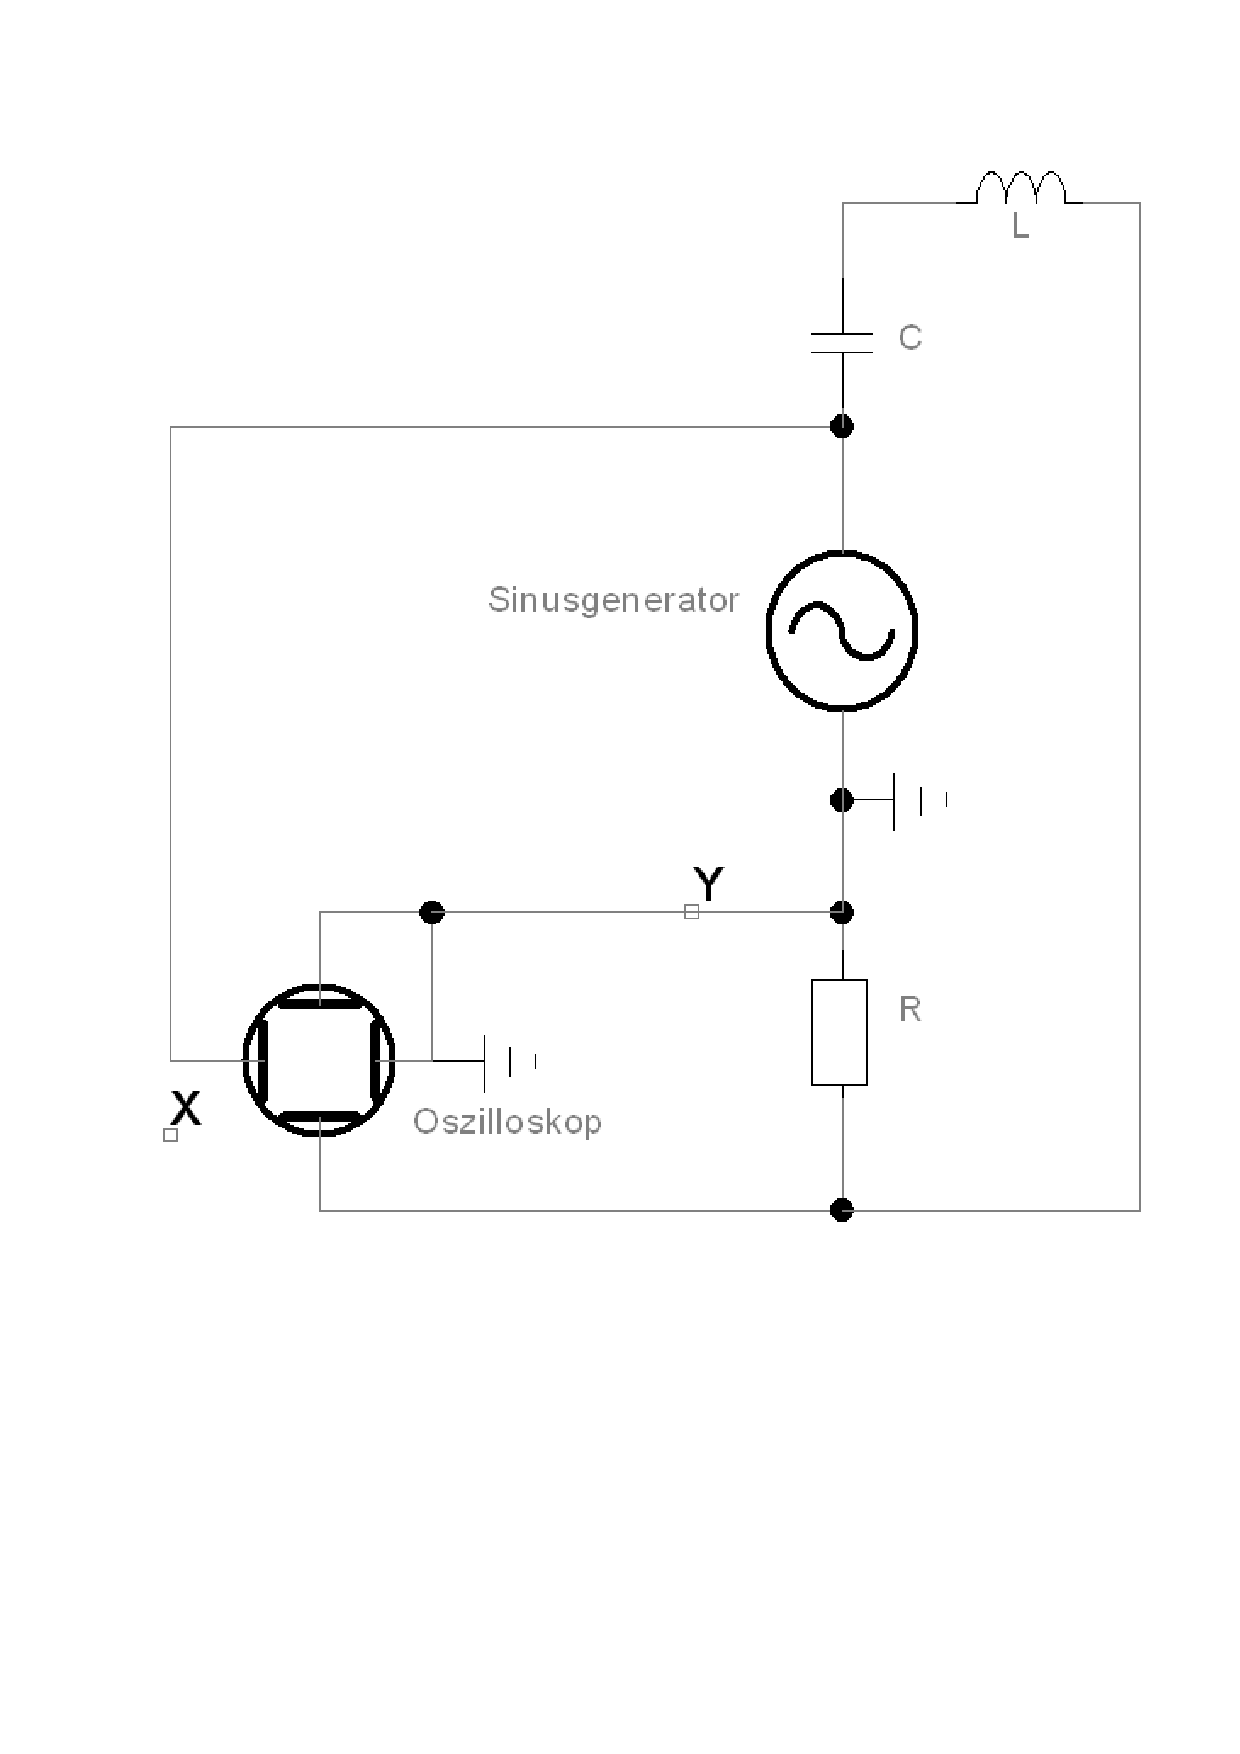
\includegraphics[width=0.5\textwidth]{plots/gekop_schw_kreis2.pdf}
    \caption{Schaltbild der Vorjustierung.}
    \label{fig:vorbereitung}
\end{figure}
Die Schaltung wird gemäß Abbildung \ref{fig:vorbereitung} aufgebaut. 
Der Sinusgenerator erzwingt die Schwingungen mit regelbarer Kreisfrequenz $\omega$ im Schwingkreis. 
Am Oszilloskop kann im XY-Betrieb die Phasenverschiebung zwischen dem Generator und des Schwingkreises anhand 
der Lissajous-Figuren abgelesen werden. 
Wie in \ref{subsec:erzwungen} erläutert, ist die zur Resonanzfrequenz gehörige Phasenverschiebung $\sfrac{\pi}{2}$.
Dies entspricht einer kreisförmigen Lissajous-Figur. 

%%%%%%%%%%%%%%%%%%%%%%%%%%%%%%%%%%%%%%%%%%%%%%%%%%%%%%%%%%%%%%%%%%%%%%%%%%%%%%%%%%%%%%%%%%%%%%%%%%%%%%%%%%%%%%%%%%%%%%%
\subsection{Messprogramm}
%%%%%%%%%%%%%%%%%%%
%%HIER schaltpülan einfügen wie Abb. 6
%%Nur statt 50 Ohm => 48 OHM
\begin{figure}
    \centering
    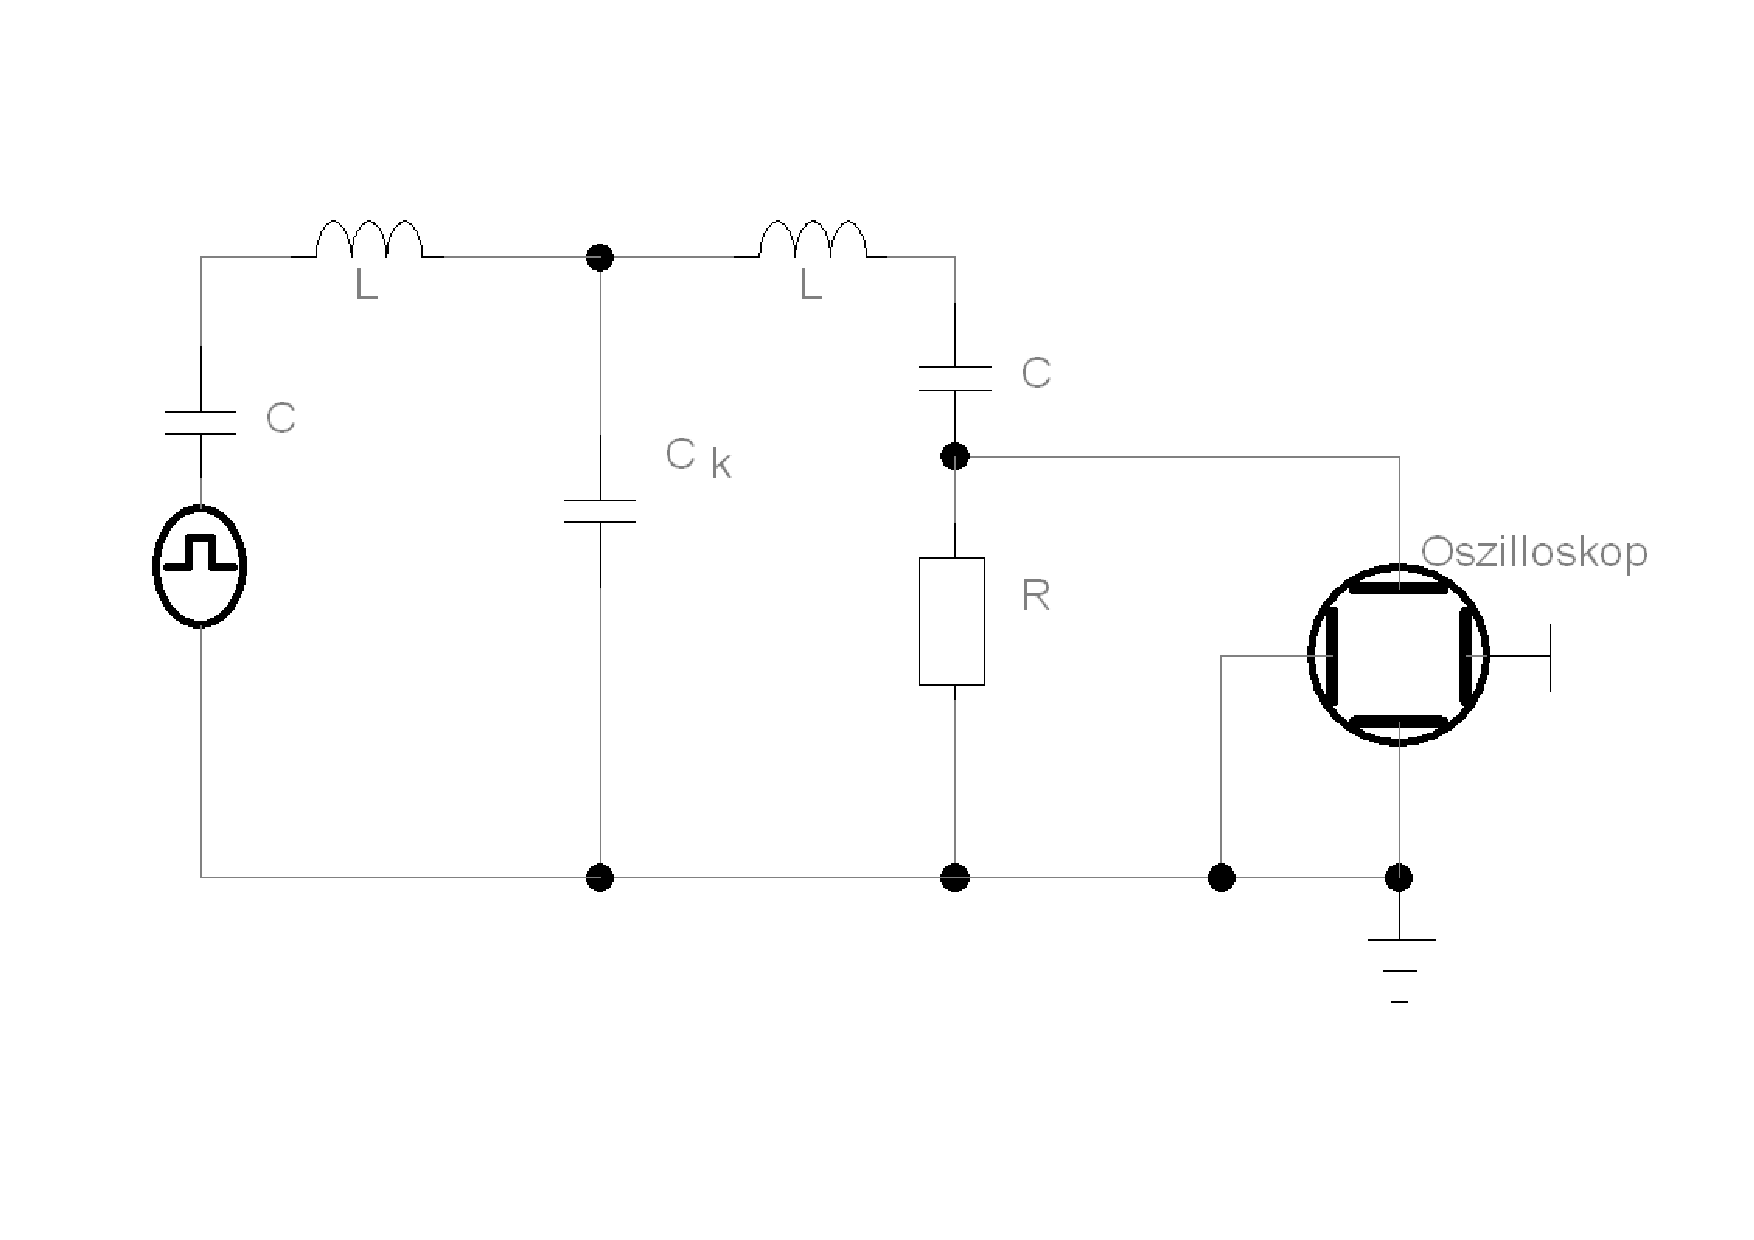
\includegraphics[width=0.75\textwidth]{plots/gekop_schw_kreis3.pdf}
    \caption{Schaltplan des Messprogramms.}
    \label{fig:messung_schweb}
\end{figure}
Zuerst wird der Schaltplan gemäß Abbildung \ref{fig:messung_schweb} aufgebaut. 
Der linke Schwingkreis soll hier über ein Rechteck-Signal des Sinus-Generators angeregt werden. 
Zum rechten Schwingkreis gelangt die Schwingungsenergie demnach ausschließlich über die gemeinsame Kopplungsleitung. 
Die über den Widerstand abfallende Spannung wird auf den Y-Eingang des Oszilloskops gelegt. 
Dort kann jetzt der zeitliche Schwingungsverlauf der Spannung verfolgt werden. 
Von Interesse sei hier das Verhältnis von Schwingungs- zu Schwebungsfrequenz. 
Hierfür sind die Schwingungsmaxima zu zählen und durch die Anzahl der Schwebungen, in denen diese Schwingungsmaxima zu finden 
sind, zu teilen. 
Dies wird für verschiedene Werte der Kopplungskapazität gemacht, die auf die festen Werte $\SI{4.7}{\nano\farad}$, 
$\SI{6.8}{\nano\farad}$, $\SI{8.2}{\nano\farad}$, $\SI{10.0}{\nano\farad}$ und $\SI{12.0}{\nano\farad}$ eingestellt werden kann.
Niedrigere Frequenzen sind zwar auch möglich, wie aus Abbildung \ref{fig:platte} ersichtlich ist, aber nicht sinnvoll. 
Die Anzahl der Schwingungen je Schwebung wäre zu gering und schwierig abzuzählen. 

Als nächstes wird der Stromkreis anstelle von Rechteck-Schwingungen mit Sinus\-/Schwingungen erregt. %latex trennt Worte mit Bindestrichen nur an diesen. Dieses Wort rutscht im pdf aus dem Blockformat. mit dem hier verwendetetn zeichen \-/ erlaubt man Latex, das Wort doch noch zu trennen 
Außerdem wird das Oszilloskop erneut auf den XY-Modus gestellt und der Generator auf die X-Achse gegeben. 
Unter Variation der Kopplungskapazität sollen nun die Frequenzen $\omega _+$ und $\omega _-$ gesucht und gemessen werden, 
also die Frequenzen, bei denen die Lissajous-Figur entsprechend einen Phasenunterschied von $0$ beziehungsweise $\pi$ indiziert. 

Zeitgleich dazu wird die über den ohmschen Widerstand $R=\SI{48}{\ohm}$ abfallende Spannung gemessen, sodass im Anschluss 
daran der entsprechende Strom mit $U=RI$ berechnet werden kann, der sich aus dem Experiment ergibt. 